\subsection{What changes when four more funds are examined?}\label{sec:breadth}
The follow-up extends QQQ, IWM, EFA and TLT to the same \BF{sessions}-session calendar as SPY. It adds \BF{newPairs} paired fund-days and reuses the \BF{reusePairs} January observations already examined. That gives \BF{pairs} pairs for the four funds and \BF{unionPairs} distinct fund-days including SPY.

The follow-up plan was fixed before downloading the additional observations, but after the SPY result was known. This is an exploratory follow-up, not untouched chronological validation. It expands the set of funds within one historical period.

The main count of affected dates excludes the previously seen January 2014 panel and the two discovery dates. That leaves \BF{eligible} eligible sessions per fund before missing measurements. The full-calendar slopes and smoothed risk calculations retain those dates to preserve time spacing and memory. The same date indices are used when resampling all funds. Shared dates are not treated as independent evidence merely because several funds are observed.

\begin{figure}[H]
\centering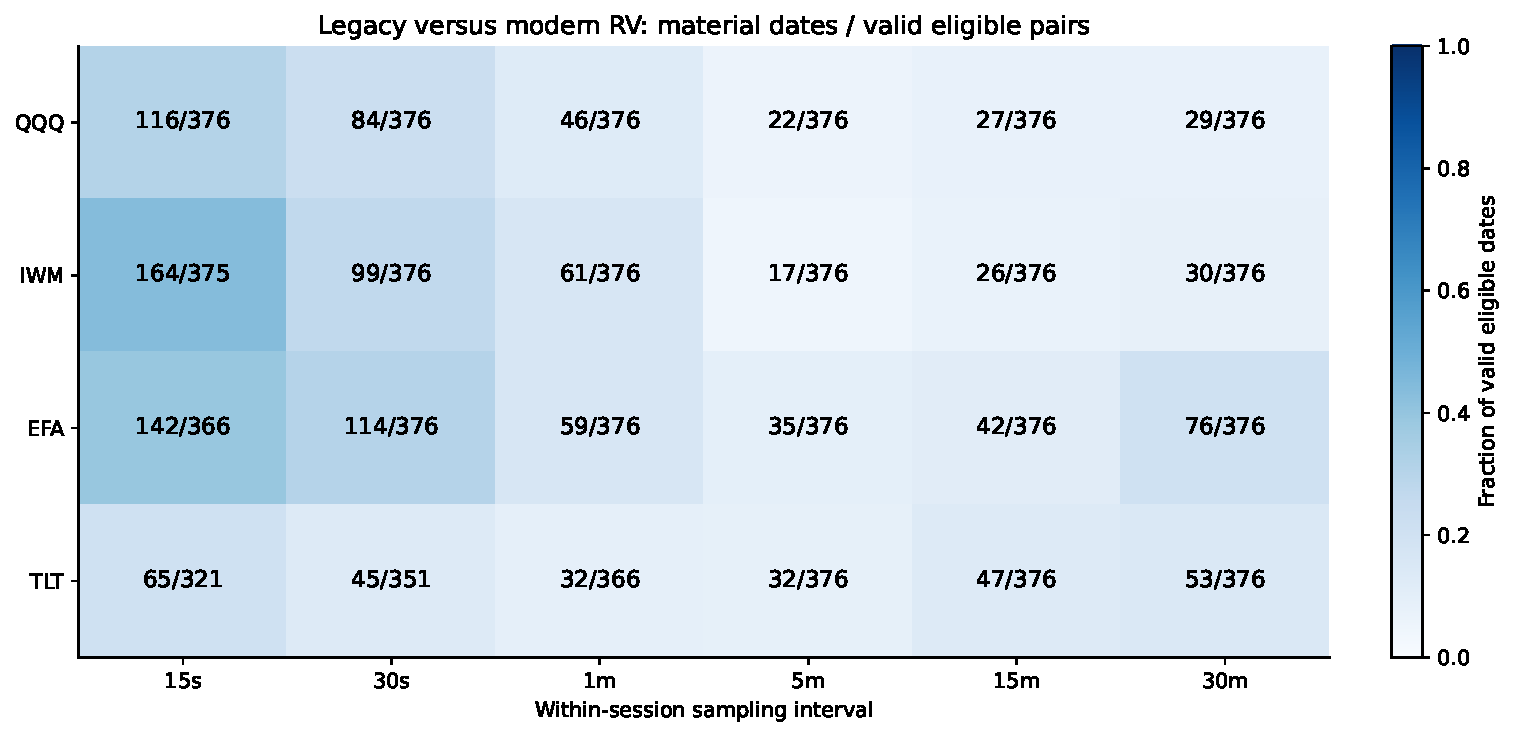
\includegraphics[width=\linewidth]{figures/breadth_incidence_rv.pdf}
\caption{Affected RV dates for every fund and sampling interval in the follow-up. Each cell gives affected dates / valid eligible pairs. Darker cells mean a larger affected fraction; the shared color scale runs from zero to one. The RV ratio must lie outside $[1/1.1,1.1]$ to count as material. Previously seen January dates and discovery dates are excluded. A missing pair does not count as agreement.}\label{fig:breadth-incidence}
\end{figure}

\textbf{How to read the complete comparison.} Table~\ref{tab:breadth-risk} places the daily measurement counts next to the later position differences. These answer different questions. RV/RQ counts concern individual eligible dates. Position gaps use the full chronological history and are evaluated after the warmup. A daily measurement difference can affect later proposals because the rule remembers past RV.

\begin{table}[H]\centering\small
\caption{All four follow-up funds at one and five minutes under the original rule. RV/RQ entries are affected dates / valid eligible dates. Capped and uncapped columns give mean absolute position gaps in percentage points. The final column counts evaluation dates with a capped gap of at least 5pp. Complete histories have \Fact{origins} evaluation dates. \emph{Withheld} means that the required TLT history is incomplete; it does not mean a zero effect.}\label{tab:breadth-risk}
\begin{tabular}{llrrrrr}\toprule
Fund & Grid & RV hits/valid & RQ hits/valid & Capped pp & Uncapped pp & Large origins \\ \midrule
QQQ & 1m & \BF{QQQ60LRVN}/\BF{QQQ60LRVD} & \BF{QQQ60LRQN}/\BF{QQQ60LRQD} & \BF{QQQ60capped} & \BF{QQQ60uncapped} & \BF{QQQ60large} \\
QQQ & 5m & \BF{QQQ300LRVN}/\BF{QQQ300LRVD} & \BF{QQQ300LRQN}/\BF{QQQ300LRQD} & \BF{QQQ300capped} & \BF{QQQ300uncapped} & \BF{QQQ300large} \\
IWM & 1m & \BF{IWM60LRVN}/\BF{IWM60LRVD} & \BF{IWM60LRQN}/\BF{IWM60LRQD} & \BF{IWM60capped} & \BF{IWM60uncapped} & \BF{IWM60large} \\
IWM & 5m & \BF{IWM300LRVN}/\BF{IWM300LRVD} & \BF{IWM300LRQN}/\BF{IWM300LRQD} & \BF{IWM300capped} & \BF{IWM300uncapped} & \BF{IWM300large} \\
EFA & 1m & \BF{EFA60LRVN}/\BF{EFA60LRVD} & \BF{EFA60LRQN}/\BF{EFA60LRQD} & \BF{EFA60capped} & \BF{EFA60uncapped} & \BF{EFA60large} \\
EFA & 5m & \BF{EFA300LRVN}/\BF{EFA300LRVD} & \BF{EFA300LRQN}/\BF{EFA300LRQD} & \BF{EFA300capped} & \BF{EFA300uncapped} & \BF{EFA300large} \\
TLT & 1m & \BF{TLT60LRVN}/\BF{TLT60LRVD} & \BF{TLT60LRQN}/\BF{TLT60LRQD} & \BF{TLT60capped} & \BF{TLT60uncapped} & \BF{TLT60large} \\
TLT & 5m & \BF{TLT300LRVN}/\BF{TLT300LRVD} & \BF{TLT300LRQN}/\BF{TLT300LRQD} & \BF{TLT300capped} & \BF{TLT300uncapped} & \BF{TLT300large} \\
\bottomrule\end{tabular}

\end{table}

\textbf{QQQ qualifies the reassuring SPY result.} At five minutes, QQQ has \BF{QQQ300large} of \BF{QQQ300origins} evaluation dates with a capped gap of at least 5pp; SPY has \Fact{large300} under the original rule. QQQ's mean capped gap is \BF{QQQ300capped}pp and its uncapped gap is \BF{QQQ300uncapped}pp. The funds use the same calendar, initial-state rule, warmup, target and cap.

Thus the SPY result cannot justify the general claim that five-minute sampling makes this source issue negligible. The comparison concerns proposed amounts from the rule. It does not measure realized losses, and the affected dates are not necessarily independent episodes.

\textbf{EFA shows the opposite problem: a small final gap hides a larger proposal gap.} At one minute, its mean absolute uncapped gap is \BF{EFA60uncapped}pp. After the cap, it is \BF{EFA60capped}pp. The cap therefore removes \BF{EFA60attenuation}\% of the mean gap. This is the same mathematical masking effect as the invented example in the reader's guide.

IWM has a larger one-minute capped gap and much less masking. For TLT, \BF{TLT60missing} eligible one-minute pairs have incomplete grids, so the specified full-history risk calculation is withheld. Dropping those dates would make nonconsecutive sessions appear consecutive and change the memory update. The study instead keeps the missingness visible.

\begin{figure}[H]
\centering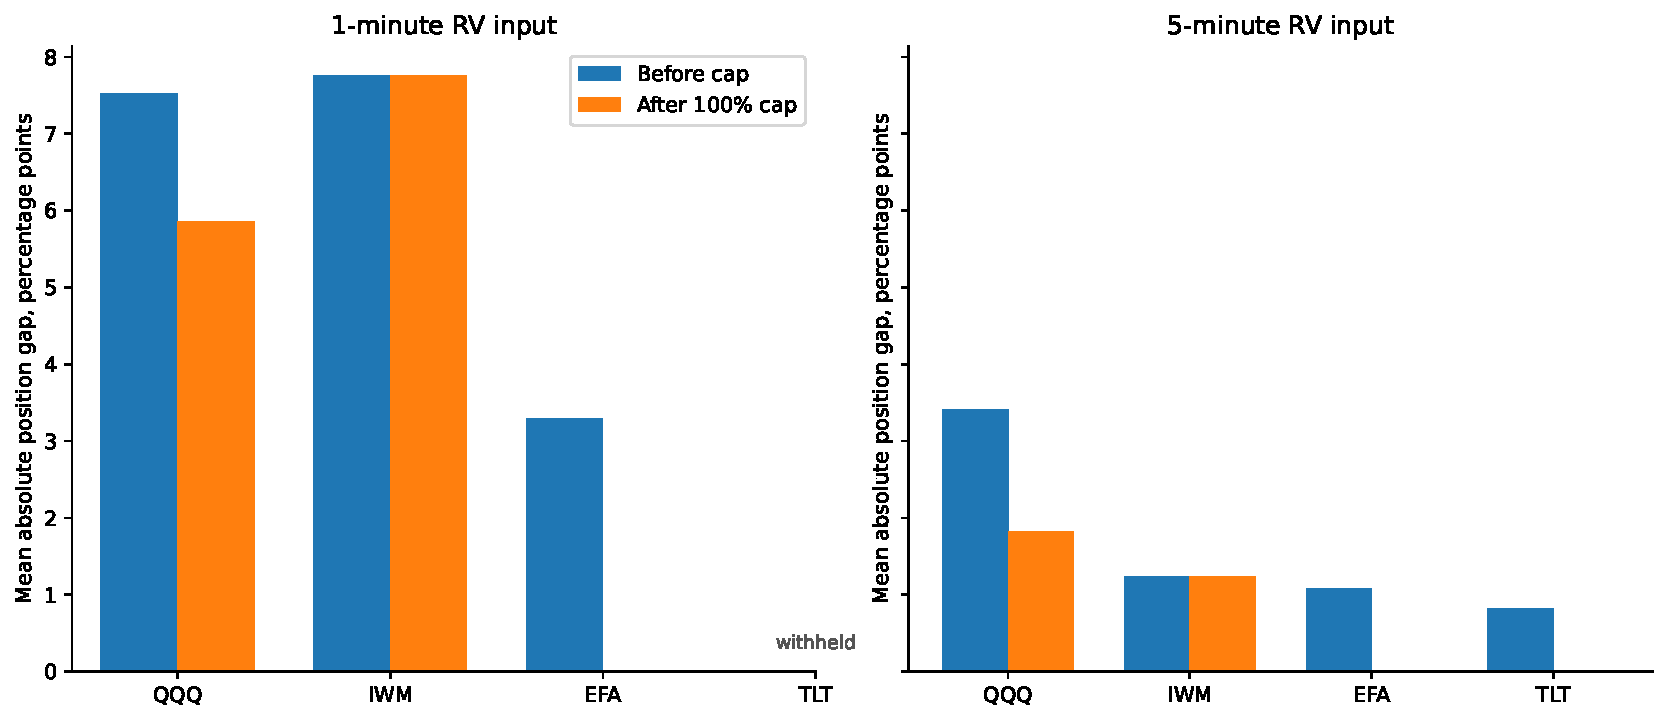
\includegraphics[width=\linewidth]{figures/breadth_cap_comparison.pdf}
\caption{Mean position gaps before and after the common cap. Both panels use the same vertical scale, measured in percentage points. The cap can hide most of the proposal gap for some funds, while leaving much more of it for others. TLT's incomplete one-minute comparison is explicitly withheld. A large percentage of masking must be read together with the actual uncapped gap. These are differences between rule inputs, not trading returns.}\label{fig:breadth-cap}
\end{figure}

\textbf{The category-B explanation is also fund-specific.} For QQQ at one minute, restoring B information leaves \BF{QQQ60BRVN} material RV dates. Using all modern condition information with legacy time leaves \BF{QQQ60CRVN}. Restoring B therefore does not explain QQQ in the same way as SPY.

This supports checking the full set of source fields and how they interact with the pipeline. It does not establish one economic cause for every fund or one universal category-based repair. The exact meanings of every field in the mounted sources remain a separate documentation question.

\textbf{Checks and complete reporting.} The export passed \BF{members} file-member hash checks, calendar and coverage checks, and daily correspondence and measurement checks. A separate result implementation recalculated \BF{checks} numerical values. It checked the smoothed rule through explicit weighted sums, separately implemented the block resampling and rejected a deliberately changed affected-date count.

Appendix~\ref{app:breadth} retains all fixed fund/grid/construction counts and their valid denominators. The supplied summary files also retain all three slope bands, all risk summaries and all specified block-length intervals. The follow-up shares the same historical source regime as SPY; these checks do not turn it into a test of a new regime or make either source verified economic truth.

